% esta si 
\documentclass{article}
\usepackage[utf8]{inputenc}
\usepackage[spanish]{babel}
\usepackage{graphicx, graphics, float, fancyhdr, titling}
\usepackage{listings, subcaption}
\usepackage[a4paper, total={6in, 9.5in}]{geometry}
\usepackage{hyperref}
\renewcommand{\footrulewidth}{0.4pt}
\title{

\includegraphics[width=1.75in]{imagenes/UGR-Logo.png} \\
\vspace*{1in}
\textbf{Práctica 4, Sesión 2} \\
Seguridad en Sistemas Operativos \\
\vspace*{0.5in}}
\author{Andrés Merlo Trujillo \\
\vspace*{0.5in} \\
E.T.S. de Ingenierías Informática y de Telecomunicación \\
\textbf{Universidad de Granada}} \date{\today}
%\date{}
\hypersetup{
    colorlinks=true,
    linkcolor=black,
}

\renewcommand\maketitlehooka{\null\mbox{}\vfill}
\renewcommand\maketitlehookd{\vfill\null}


\begin{document}
\begin{titlingpage}
\maketitle
\end{titlingpage}

\newpage

\tableofcontents

\newpage

\pagestyle{fancy}
\fancyhead[L]{Andrés Merlo Trujillo}
\fancyhead[R]{Seguridad en Sistemas Operativos}
%\addcontentsline{toc}{section}{Ejercicio 1}
%\section{Ejercicio 1}
%\begin{figure}[H]
%    \centering
%    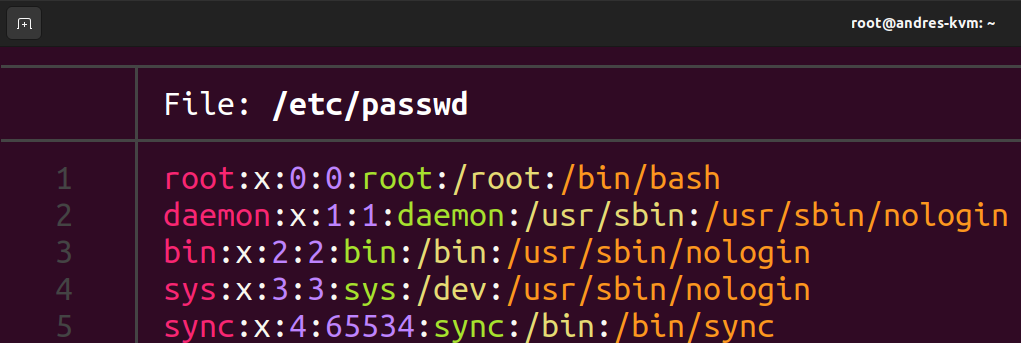
\includegraphics[width=\textwidth]{imagenes/passwdfile.png}
%\end{figure}

\section{Ejercicio 1}

Antes de nada hay que saber la version exacta del kernel para poder instalar el paquete \verb|linux-headers|, para ello, se usa el comando \verb|uname -r|:

%salida comando
%caption: Version del kernel que está usando mi distribucion

Ahora lo que hay que hacer es instalar \verb|LiME| siguiendo las instrucciones proporcionadas en el guion de practicas. Una vez instalado, como es en maquina local, se ejecuta el comando \verb|sudo insmod lime-5.15.0-56-generic.ko path=/home/usuario/evidencias/volcado101 format=raw|

%foto
%caption: Volcado de memoria realizado.

Y ahora si nos vamos al directorio \textit{evidencias} deberia aparecer lo siguiente:

%foto del archivo
%caption: Volcado de memoria realizado correctamente.

\section{Ejercicio 2}

Antes de nada hace falta instalar \verb|volatility| y descargarse la imagen RAM de PRADO. %Tambien cabe destacar que los paqeutes \verb|python python-crypto| han sido sustituidos por \verb|python3 python3-cryptography|.

\subsection{¿A qué sistema operativo corresponde la imagen?}

Primero, para comprobar si usa Linux, se usa el comando \verb|strings memory.img | grep -i "Linux version" | uniq|, en caso de no devolver nada, es otro sistema operativo, seguramente Windows.

%foto para windows
%caption: salida para un so distinto de linux

En cambio, con la imagen del ejercicio anterior sale lo siguiente:

%foto de la slaida
%caption: aqui si aparecen referencias


Y ahora, usando el comando \verb|vol.py -f memory.img imageinfo| se puede intuir que sistema operativo utiliza:

%foto
%caption: Salida del comando.

Como se puede ver, está usando Windows y por los perfiles sugeridos, parece ser que está usando Windows 7 o Windows Server 2008.

\subsection{Listar los procesos en ejecución en el momento de la adquisición.}

Usando la orden \verb|vol.py -f memory.img --profile=Win7SP1x64 pslist| se puede obtener esa informacion:

%foto de eso
%caption: Salida del comando.


\end{document}
